% !TEX root = ../Main.tex
\chapter{外接球：球心定位}

\textbf{外接球}是\textbf{外接圆}的三维版本：球面过多面体的每一个顶点——球心到各顶点的距离都相等。

\section{外接圆与外接球}

\state{两个平行的刻画}{
    \begin{itemize}
        \item \textbf{外接圆}：圆心到各顶点的距离都相等 $\Rightarrow$ 圆心是\textbf{各边中垂线的交点}。
        \item \textbf{外接球}：球心到各顶点的距离都相等 $\Rightarrow$ 球心是\textbf{各边中垂面的交点}。
    \end{itemize}
}

\begin{center}
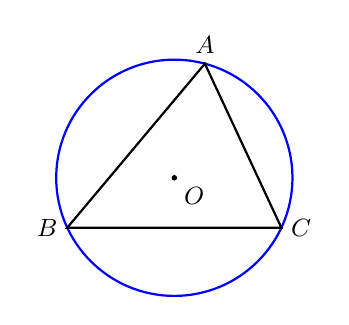
\begin{tikzpicture}[scale=1]
    \draw[thick, blue] (0,0) circle (1.5);
    \coordinate (A) at ({1.5*cos(75)},{1.5*sin(75)});
    \coordinate (B) at ({1.5*cos(205)},{1.5*sin(205)});
    \coordinate (C) at ({1.5*cos(335)},{1.5*sin(335)});
    \draw[thick] (A) -- (B) -- (C) -- cycle;
    \fill (0,0) circle (1pt) node[below right] {\small $O$};
    \node at (A) [above] {\small $A$};
    \node at (B) [left] {\small $B$};
    \node at (C) [right] {\small $C$};
\end{tikzpicture}
\end{center}

\section{球心与截面圆心的关系}

取多面体的\textbf{某一个面}，这个面的顶点在该面内有自己的外接圆，圆心记作 $O'$。球心 $O$ 与 $O'$ 之间有如下关系。

\state{球心 $O$ 与某截面外接圆圆心 $O'$}{
    设多面体某一个面在平面 $\alpha$ 内，该面顶点的外接圆圆心为 $O'$。则
    \begin{enumerate}
        \item[(1)] $OO'\perp\alpha$——\textbf{球心到截面圆心的连线垂直于该面}；
        \item[(2)] 若该面恰好过球心，则 $O$ 与 $O'$ \textbf{重合}。
    \end{enumerate}

    道理：$O$ 到该面上各顶点距离都是 $R$，把 $O$ 投影到 $\alpha$ 上得垂足 $O'$，则 $O'$ 到这些顶点的距离也都相等（都等于 $\sqrt{R^2-OO'^2}$），所以 $O'$ 正是它们的外接圆圆心，且 $OO'\perp\alpha$。
}

由此求外接球：\textbf{先在一个面里定出外接圆圆心 $O'$，过 $O'$ 作该面的垂线，球心 $O$ 在这条垂线上}；再用"$O$ 到各顶点等距"列方程求出半径。
